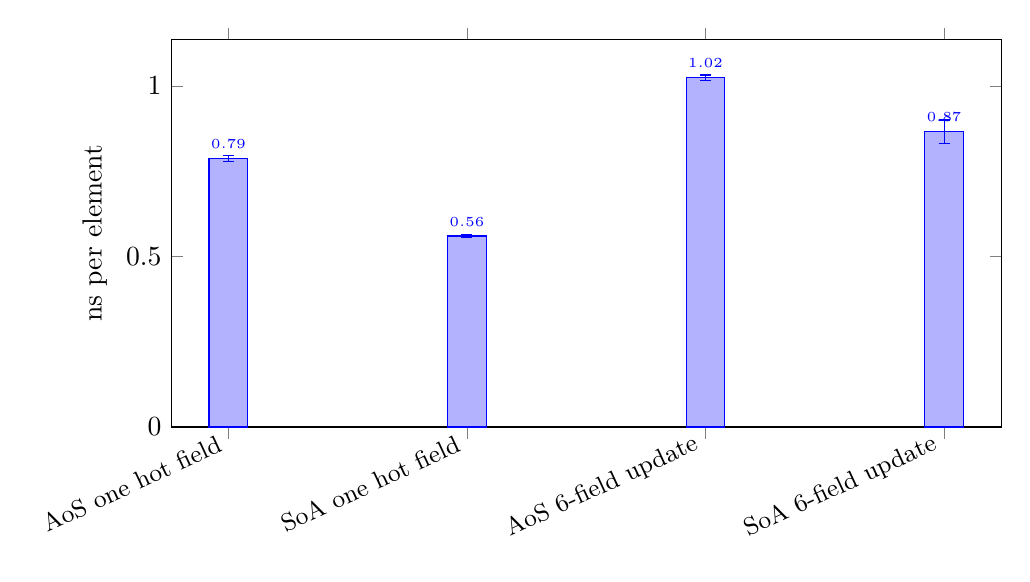
\begin{tikzpicture}
\begin{axis}[ybar, width=\textwidth, height=6.5cm, bar width=14pt, ymin=0, symbolic x coords={AoS one hot field,SoA one hot field,AoS 6-field update,SoA 6-field update}, xtick=data, x tick label style={rotate=25, anchor=east, font=\small}, ylabel={ns per element}, enlarge x limits=0.08, legend style={font=\small, at={(0.98,0.98)}, anchor=north east}, nodes near coords, nodes near coords style={font=\tiny}, every node near coord/.append style={/pgf/number format/.cd, fixed, precision=2}]
\addplot+[error bars/.cd, y dir=both, y explicit] coordinates {(AoS one hot field,0.7873) +- (0,0.0086) (SoA one hot field,0.5600) +- (0,0.0043) (AoS 6-field update,1.0246) +- (0,0.0077) (SoA 6-field update,0.8660) +- (0,0.0344)};
\end{axis}
\end{tikzpicture}